%!TEX root = ../thesis.tex
%*******************************************************************************
%****************************** Second Chapter *********************************
%*******************************************************************************

\chapter{Background}
% \ifpdf
\graphicspath{{Chapter2/Figs/Raster/}{Chapter2/Figs/PDF/}{Chapter2/Figs/}}
% \else
%     \graphicspath{{Chapter2/Figs/Vector/}{Chapter2/Figs/}}
% \fi
In this chapter we will take a deeper dive into the issues around education and e-learning that
is relevant to this project, and

\section{Literature Review in Education and e-Learning}

Identifying issues in traditional higher education today that a blockchain-based system can better
tackle is one of the objectives of this project. This informs the scope of the
project and the design of the deliverables.

There is an abundant amount of pedagogy and learning method research, which focuses on the
instruments and mode of delivery. These include methods such as "scaffolding", "constructivism",
"problem-based learning", and "active learning" \citep{ali2005effective}. However, this
research area is considered out of the scope of discussion for this project, which does not
aim to provide new insight into ICT-enhanced pedagogies. Instead, this project is interested in
mapping components of e-learning, such as delivery, assessment, and record keeping
in a more general-purposed, pedagogically neutral manner to a blockchain.

\subsection{Assessments and Transparency}

Assessment is arguably the most important process in the business of education as it "drives what
is learnt and taught" and "converts learning into credentials". \citep[p.160]{campbell2010digital}

\citet{brown1999assessment} summarises examples of popular sentiments learners held about both
continuous assessments and traditional exams, such as:

\begin{enumerate}
	\setlength\itemsep{0em}
	\item Assessment tasks do not increase students' want to learn, only their need to learn, promoting unhappiness;
	\item Invalid and unreliable marking due to speed or fatigue of assessors, plagiarism and unwanted collaborations, etc.;
	\item Sub-optimal levels of feedback after many types of assessments;
	\item Students feel forced into surface learning.\\
	      \citep[p.62-65]{brown1999assessment}
\end{enumerate}

The importance of assessments, coupled with popular unhappiness and mistrust amongst learners towards
them, increases the tension between the teacher (or educational provider) and the learners.

\citet{suhre2013determinants} looks into motivation on study progress in a higher education setting by collecting data
from 168 first-year university students for six months. The study found three main factors that motivates academic
progress: intrinsic abilities, personal motivations such as a need to achieve or fear of failure, and transparency in
exams and assessments.

Transparency here refers to both the clarity of assessment goals and the procedures for assessing these goals.
It should be clear to learners what knowledge is required for a sufficient level of mastery \citep{suhre2013determinants}.
The difference this makes was significant:

\begin{itemize}
	\setlength\itemsep{0em}
	\item Students' perceptions of degree programme organisation and transparency of exams are
	      significantly correlated with academic performance;
	\item Academic pressure is substantially influenced by the perceived transparency of assessments.
\end{itemize}

The earlier [p.100]\citet{bryan2006innovative} research echoed the same argument, that students realise their full potential
when they understand the assessment task, marking criteria and expected standards.

An improvement in the transparency of goals, procedures, knowledge required of assessments 
can directly tackle some of the negative sentiments listed above from \citet{brown1999assessment}. 
The design of the blockchain schema and Smart Contracts should involve these as required parameters, and also an increase
in feedback.

\subsection{Personalisation in Education}

% [TODO: Cover personalisation broadly and in terms of curriculum (which modules to take,
% 	customised passing thresholds) which can be negotiated on the blockchain.
% 	To be added if there is time for the project to cover this area.]

Personalisation is regarded as the solution to traditional bureaucratic state education that is irresponsive,
inflexible, over-regulated, with the ‘one size fits all’ approach \citep{bragg2014review}. 
Research points to a growing appreciation of the need to support and
encourage learner control over the whole/entire learning process \citep{dron2007designing}.

Current research into personalisation (or customisation) of education is broad and covers both the personalisation
of pedagogy and curriculum. 

\citet{green2005futurelab} summarised four key areas pivotal to enabling personalised learning through digital
technologies. The technologies should:

\begin{itemize}
	\setlength\itemsep{0em}
	\item ensure that learners are capable of making informed educational decisions;
	\item diversify and recognise different forms of skills and knowledge;
	\item create diverse learning environments; and
	\item include learner focused forms of feedback and assessment.
\end{itemize}

The design of a learning platform that aims at supporting personalisation must therefore focus on facilitating these
actions. For example, providing support to students who are choosing their personalised curriculum, and 
providing maximal diversity in knowledge by creating an open, global course catalogue that is 
multi-disciplinary and cross-institutional.

% https://www.researchgate.net/publication/262901454_Education_%27consumerism%27_and_%27personalisation%27

% (p.7)

% http://onlinelibrary.wiley.com/doi/10.1111/j.1467-8527.2008.00411.x/full

\subsection{e-Learning Systems}

E-learning has been growing as an industry and research area, and the Learning Technology Standards Committee
was set up within the IEEE Computer Society to devise relevant standards. In 1999, the Learning Technology
Systems Architecture (LTSA) standard was published (See Figure \ref{fig:LTSA}) and was last revised in 2003.

\begin{figure}[!ht]
	\centering
	\includegraphics[width=1.0\textwidth]{ltsa2003}
	\caption[Learning Technology Systems Architecture]
	{Learning Technology Systems Architecture, IEEE Standard \citep[p.9]{ieee2003ltsa}}
	\label{fig:LTSA}
\end{figure}

LTSA is "pedagogically neutral, content-neutral, culturally neutral, implementation-neutral,
and platform-neutral"\citep[p.1]{ieee2003ltsa}. It provides a valuable way of organising
the scope and discussion in this project. It identified four main components: learner entity, coach,
delivery, evaluation; two main stores: learning resources, learner records; and the information flows
or actions between them.

Identifying the properties of a blockchain-based system that could improve these components, stores and
flows is critical to this project. For example, the distributed, immutable storage of learner records could
provide extra security.

% \subsection{e-Learning Research Framework}

% \citet{garrison2011learning} provided a framework for research and practice called the "Community 
% of Inquiry (CoI)" framework, which included three main categories:

% \begin{enumerate}
%     \setlength\itemsep{0em}    
%     \item Enhancing the social presence, such as collaborative learning
%     \item Enhancing the cognitive presence, such as practical inquiry and critical thinking
%     \item Enhancing the teaching presence, especially with asynchronous e-Learning (eg. pre-recorded lectures)
% \end{enumerate}

% A blockchain back-end could potentially provide experiential improvements in the above three categories as well. 
% For example, Smart Contracts could enhance the social and teaching presence by facilitating teacher-learner, or 
% learner-learner negotiations.

% \subsection{Self-Regulation and Motivation}

% There are several dimensions of self-regulation that will help a learner stay on an 
% e-Learning course or curriculum:

% \begin{table}[!ht] 
%     \caption{Self-Regulation and Motivation Strategies, adapted from \citep[p.189]{o2013web}}
%     \centering
%     \label{table:Self-regulation Dimensions}
%     \begin{tabular}{l c }
%         \toprule
%         Self-regulation Dimensions & Examples of Motivation Strategies \\ 
%         \midrule
%         Motives & Setting challenging but achievable goals \\ \hline
%         Methods of Learning & Summarisation, outline-formatted notes, \\
%         & interrogation and rehearsal, etc\\ \hline
%         Time Management & Prioritizing tasks, dealing with procrastination\\ \hline
%         Physical Environment & An environment conducive to learning\\ \hline
%         Social environment & Help seeking: knowing when help is needed,\\
%         & identifying sources of help, framing help request,\\
%         & evaluating help received\\ \hline
%         Performance & Observing and reflecting upon performance\\
%         & with short-term and long-term goals\\
%         \bottomrule
%     \end{tabular}
% \end{table}

% An e-learning programme should equip a learner with these self-regulation skills,
% and the e-learning system should provide tools that facilitate and enable the 
% motivation strategies.

\section{Security and Privacy}

The security of e-learning systems have also been a concern. For example, \citet{el2003privacy} noted that “while many
advances have been made in the mechanics of providing online instruction, the needs for privacy and security have to-date
been largely ignored. At best they have been accommodated in an ad-hoc, patchwork fashion.”

The consequences of cybersecurity breaches have also become more and more expensive. For example, when the General Data
Protection Regulation (GDPR) comes into effect across Europe in May 2018, the maximum fine for poor practices and data
breaches will be £17 million or 4\% of global turnover \citep{ico2017gdpr}.

The scale and severity of historic breaches of of internet services has been worrying. Most notably in the e-learning
industry, the education platform Edmodo was hacked and 77M account details were lost and on sale on the dark
web, endangering students, teachers and parents who are account holders \citep{opsecmonkey2017edmodo}.

The sizable threat and consequences makes a "security by design" and "privacy by design" approach for future 
systems very important. A secure data storage such as blockchains could add massive value to e-Learning systems.
% The Information Commissioner's Office also encourages a "privacy by design approach" and 
% https://www.ipc.on.ca/resource/privacy-by-design/

\section{Properties of Blockchain Technologies}

The advent of cryptocurrencies made blockchains an overnight darling, set to make significant disruptions
in several industries such as financial services, currency exchanges, supply chain management, retail
advertising and identity management \citep{forbes2017industries}.

The blockchain data structure is a timestamped list of blocks, which stores data about transactions
that occur within the blockchain network. It only allows the insertion of transactions, not the update
or deletion of existing transactions. Its ability to prevent tampering is known as "immutability". \citep[p.182]{xu2016blockchain}

Blockchains can be classified into two types: one being a permissionless (public) blockchain which anyone can
use and no central authority exist to allow or ban peers; the other a permissioned blockchain (can be public or private)
where a central entity assigns read/ write rights to individual peers \citep[p.1]{wust2017you}. Table \ref{table:permvsless}
summarises the main differences in these two types of blockchain.

%https://eprint.iacr.org/2017/375.pdf
\begin{table}[!ht]
	\caption[Comparison of permissioned and permissionless blockchains]
	{Comparison of permissioned and permissionless blockchains, modified from \citet[p.3]{wust2017you}}
	\centering
	\label{table:permvsless}
	\begin{tabularx}{\textwidth}{>{\bfseries}lXX}
		Properties    & Permissioned blockchains                                                                           & Permissionless blockchains                     \\
		\toprule
		Speed         & Low throughput and slow latency                                                                    & high throughput and medium latency             \\\midrule
		Peers         & High number of both readers and writers                                                            & High number of readers, small group of writers \\\midrule
		Consensus     & Proof of work or proof of stake by miners                                                          & BFT protocols such as PBFT                     \\\midrule
		Central                                                                                                                                                             \\Authority & No & Yes\\\midrule
		Privacy       & Can be achieved using cryptographic techniques but typically comes at the cost of lower efficiency &
		Reading rights can be restricted by central authority, readers and writers can also run separated parallel blockchains that are interconnected.                     \\\midrule
		Verifiability & \multicolumn{2}{c}{Observers can verify the state of the blockchain}                                                                                \\\midrule
		Redundancy    & \multicolumn{2}{c}{High, provided through replication across the peers}
		\\\bottomrule
	\end{tabularx}
\end{table}

Using blockchains as a data storage gives the system a very high degree of integrity. The public verifiability,
redundancy (in Table \ref{table:permvsless}) and immutability of the blockchain makes it very difficult to
corrupt or lose the data stored.

\subsection{Decision Framework for Blockchain Solutions}

\begin{figure}[!ht]
	\centering
	\includegraphics[width=1.0\textwidth]{blockchain_need}
	\caption["Do you need a blockchain?" flowchart]
	{"Do you need a blockchain?" flowchart \citep[p.3]{wust2017you}}
	\label{fig:blockchain_need}
\end{figure}

\citet[p.3]{wust2017you} proposed a decision flowchart (Figure \ref{fig:blockchain_need}) to determine whether a blockchain is
the appropriate solution for a problem, and which type of blockchain is the most appropriate. Here is an analysis of our problem at
hand with the decision flowchart steps:

\begin{enumerate}
	\item \textbf{Do you need a store state?} Yes. Records in an e-learning system require secure storage.
	\item \textbf{Are there multiple writers?} Yes. There are many different authorities, institutions, educators and learners
	      involved in an e-learning blockchain that demands write assess into records.
	\item \textbf{Can you use an always online Trusted Third Party (TTP)?} \citet[p.2]{wust2017you} described two options of
	      using a TTP: delegate write operations completely to the TTP if it is always online so that it verifies all state
	      transitions, or use the TTP as a certificate authority in the setting of a permissioned blockchain if the TTP is usually
	      offline.\\
	      In the e-learning context, a TTP could be the e-learning platform provider. However, the delegation of write operations
	      to the platform goes against modern principles of autonomy and independence for higher education institutions.
	      Governmental education ministries in most modern states audits and regulates higher education without writing student
	      records or conferring degrees. An always online TTP should not be used in order to replicate the real world context. This
	      project will answer no for this step.
	\item \textbf{Are all writers known?} Yes. Users of the system should be registered and not be anonymous to the system
	      administrators. [TODO: Why? Are there arguments to anonymous education?]
	\item \textbf{Are all writers trusted?} No. Malpractices from education institutions can occur, especially in the private,
	      for-profit sector. In a future open e-learning market, it could also be possible for anyone to start offering education
	      services. We cannot assume that all writers are trusted.
	\item \textbf{Is public verifiability required?} Yes. One of the objectives of this project is to boost trust in e-learning
	      credentials by increasing public verifiability of education journeys, increasing public accountability especially for
	      stakeholders such as employers and postgraduate studies providers.
\end{enumerate}

This process led to the recommendation of a \textbf{public permissioned blockchain} for this project.

\subsection{Properties of Smart Contracts}
Smart Contracts are self-executing code embedded in a blockchain that defines the rules and penalties around an agreement and
could automatically enforce those obligations. They can effectively "cut out the middleman" to save time, and prevent disagreements
about transactions \citep{gulhane2017ibm}. The term "chaincode" is also used interchangeably as a synonym for
Smart Contracts \citep[p.6]{valenta2017comparison}.

There are three main properties of Smart Contracts \citep[p.16]{swan2015blockchain}:

\begin{itemize}
	\setlength\itemsep{0em}
	\item \textbf{Autonomous}: after launching and running, no further communication is required between a Smart Contract
	      and its initiating agent;
	\item \textbf{Self-sufficient}: a Smart Contract should have the ability to keep itself alive when it needs to be,
	      such as raising funds by providing services, and spending them on computing power or storage;
	\item \textbf{Decentralised}: a Smart Contract does not exist on a single server, they are distributed and self-executing
	      across all of the blockchain peers.
\end{itemize}

These properties ensure effective operation of the logic defined. In an e-learning context, this can potentially
be used to govern how teaching, evaluation and feedback take place, enhancing protection for the consumers/ learners. 
It could also automate more administrative work, reducing middlemen and manual errors.

An increasing amount of research has also been focused on automating the marking process. For example, \citet{al2012auto} has run 
an experiment on using a programme to grade university project proposals and provide formative feedback. The programme was 
able to give intensive feedback, with plagiarism and grammar checks, and a semantic analysis on the quality of ideas.
This shows that as marking programs become more mature, they could have a place in assisting teachers and students. 
It could also make educational Smart Contracts extremely powerful.

By formalising assessments into a series of transparent steps executed by a peer network, this project also hopes to 
reduce the tension and disagreements between teachers and students.

\section{Overview of Blockchain Development Toolkits}

This project will involve the design of Smart Contracts for e-Learning transactions and building a demonstrator
network and applications. A review of the popular blockchain implementations and development toolkits on the
market is necessary. See Table \ref{table:blockchainscomparison} for a overview and below for more commentary.

\begin{table}[!ht]
	\caption[Comparison of key blockchain implementations, eg. Ethereum, Fabric, R3]
	{Comparison of key blockchain implementations, adapted from \citet{ibm2018hyperledger} and \citet{valenta2017comparison}}
	\centering
	\label{table:blockchainscomparison}
	\begin{tabularx}{\textwidth}{>{\bfseries}lXXXX}
		\toprule
		                & \textbf{Bitcoin}       & \textbf{Ethereum}                 & \textbf{Hyperledger Fabric}   & \textbf{R3 Corda}     \\
		\midrule
		Governance      & Bitcoin                & Ethereum                          & Linux                         & R3                    \\
		                & developers             & developers                        & Foundation                                            \\
		\midrule
		Cryptocurrency  & bitcoin                & ether, and                        & none, or                      & none                  \\
		                &                        & user-created cryptocurrencies     & user-created cryptocurrencies &                       \\
		\midrule
		Network         & permissionless, public & permissionless, public or private & permissioned, private         & permissioned, private \\
		\midrule
		Transactions    & anonymous              & anonymous or                      & public or                     &                       \\
		                &                        & private                           & confidential                  &                       \\
		\midrule
		Consensus       & proof of work          & proof of work                     & PBFT                          & PBFT                  \\
		\midrule
		Smart Contracts & none                   & yes (Solidity,                    & yes (chaincode)               & yes (chaincode)       \\
		                &                        & Serpent, LLL)                                                                             \\
		\hline
		Language        & C++                    & Golang, C++,                      & Golang, Java,                 & Kotlin, Java,         \\
		                &                        & Python                            & JavaScript                    & legal prose           \\
		\bottomrule
	\end{tabularx}
\end{table}

Bitcoin is included in the Table only as a point of reference. Building with the bitcoin
blockchain is not considered for this project because of its lack of support for Smart
Contracts (any kind of embedded logic or programmes).

\subsection*{Ethereum}

Ethereum is famous for its Turing-complete Smart Contracts capabilities, which allows entire
decentralised applications (dApps) to run autonomously on its blockchain. It has a build-in cryptocurrency
"Ether", which is used to reward miners that contribute to consensus, and to pay transaction fees.
Developers of dApps can also issue their own currency inside their Smart Contracts.

\citet[p.3-4]{valenta2017comparison} noted that compared with Ethereum, which makes records accessible
to all participants, permissioned blockchains such as Fabric and Corda provide "more fine-grained access
control to records and thus enhance privacy".
They also achieves higher performance due to a faster consensus mechanism that does not involve mining.

For this project, another crucial consideration against the adoption of the Ethereum environment is the
lack of a central authority, which makes it impossible for the platform to kick unscrupulous actors off
the blockchain.

\subsection*{Hyperledger Fabric}

\citet[p.7]{valenta2017comparison} described Fabric as a highly flexible "versatile toolbox". It
has different roles for peers within the network, where they can act as clients (end users), peers
(record keepers), endorsers (transaction verifiers), or orderers (transaction requester). The
consensus mechanism is by default a Byzantine fault-tolerant (BFT) algorithm and can be customised.
A cryptocurrency is not required, but could be developed with chaincode.

\subsection*{R3 Corda}

Built following use cases in the financial industry, Corda notably augmented Smart Contracts
with legal prose, making it a great tool for highly regulated environment. The development of
a cryptocurrency is not intended or supported. \citep{valenta2017comparison}

Education is not a highly regulated environment in most countries and this unique selling point of
Corda is not immediately attractive to this project.

\section{Existing Efforts in Blockchain for Education}

% chapter 1
% The potential of blockchain enabled systems in education has been noted by the community, with \citet[p.62]{swan2015blockchain} 
% proposing that “learning Smart Contracts could automatically confirm the completion of learning modules through standardized 
% online tests”. Appropriate configurations in permissions and visibility can also provide improved security and privacy to e-Learning.

Several blockchain-based projects for education exists. Here we look at three that has attracted plenty of media attention:
Blockcerts, Sony Global Education (GED) Blockchain, and the OpenLearn Blockchain. See Table \ref{table:existingprojects} for a quick comparison.

\begin{table}[!ht]
	\caption[Comparison of existing projects: Blockcerts, Sony GED, and OpenLearn]
	{Comparison of existing projects: Blockcerts \citep{blockcerts2018}, Sony Global Education Blockchain \citep{sonyged2017}, and the OpenLearn Blockchain \citep{openlearn2018}}		 
	\centering
	\label{table:existingprojects}
	\begin{tabularx}{\textwidth}{|>{\bfseries}p{3.3cm}|p{2cm}|X|}
		\hline
		Project                                 & Based on            & Features                                                                                   \\
		\hline
		Blockcerts \newline by MIT Media Lab             & Bitcoin             & Education providers can store a batch of certificates by paying for a bitcoin transaction,
		storing data in the OP\_RETURN transaction field on the global bitcoin blockchain.                                                                         \\
		\hline
		Sony GED \newline Blockchain                     & Hyperledger \newline Project & Developers at education institutions can use their application program interface (API) to
		securely store learning history data and certificates, integrating with third party e-Learning systems.                                                    \\
		\hline
		OpenLearn \newline Blockchain \newline by Open University & Ethereum            & An experimental plugin for Moodle, a popular course management system, is provided. \newline 
		Achievement badges can be stored on the Ethereum blockchain. Students can register for courses and receive badges in a "Student Learning Passport".\\
		\hline
	\end{tabularx}
\end{table}

% \subsection{Blockcerts}

% Blockcerts is an open standard for blockchain certificates led by MIT’s Media Lab. Education providers can use it to store
% the records of certifications they have awarded (See Figure \ref{fig:blockcerts}). One bitcoin transaction is performed for
% every batch of certificates, with the certificates stored in the OP\_RETURN transaction field on the bitcoin blockchain.
% This is paid for by the certificate issuer. \citep{blockcerts2018}

\begin{figure}[!ht]
	\centering
	\includegraphics[width=0.7\textwidth]{blockcerts}
	\caption[How Blockcerts work]
	{How Blockcerts work \citep{blockcerts2018}}
	\label{fig:blockcerts}
\end{figure}

% \subsection{Sony Global Education Blockchain}% https://blockchain.sonyged.com/

% The Sony Global Education Blockchain is based on the Hyperledger project, an open source distributed ledger
% for businesses. It provides an application program interface (API) for developers at education institutes,
% allowing integration with third party applications. It aims to provide tamper-proof, secure storage of
% learning history data for institutions. \citep{sonyged2017}

% \begin{figure}[!ht]
% 	\centering
% 	\includegraphics[width=0.7\textwidth]{sonyged}
% 	\caption[Sony Global Education Blockchain]
% 	{Operation Example of the Sony Global Education Blockchain \citep{sonyged2017}}
% 	\label{fig:sonyged}
% \end{figure}

% \subsection{OpenLearn Blockchain}% http://blockchain.open.ac.uk/

% \begin{figure}[!ht]
% 	\centering
% 	\includegraphics[width=0.95\textwidth]{openlearn}
% 	\caption[OpenLearn Blockchain scenario]
% 	{A typical education scenario with the OpenLearn Blockchain \citep{openlearn2018}}
% 	\label{fig:openlearn}
% \end{figure}

\subsection{Novelty of the Proposed Project}

\begin{figure}[!ht]
	\centering
	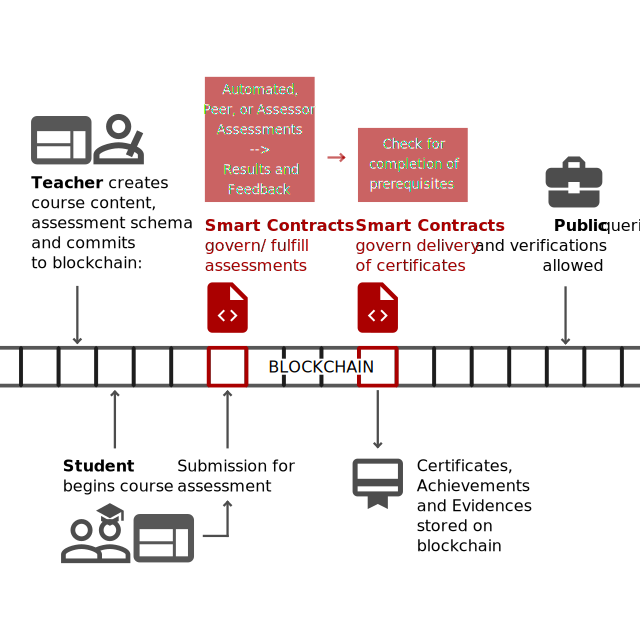
\includegraphics[width=0.95\textwidth]{moocon}
	\caption[Assessment Smart Contracts Concept]
	{Original diagram providing a high level view of how the project proposes automating assessments
		with Smart Contracts}
	\label{fig:moocon_assess}
\end{figure}

All of the above three notable efforts focus on identity management and record keeping for education.
This project will aim to extend these efforts by proposing Smart Contracts that automate assessments
(See Figure \ref{fig:moocon_assess}) and facilitate the negotiation of personalised curricula.

The vision of this project will also be to create an e-Learning marketplace that teachers can use directly,
instead of a blockchain network that education providers will have to consume through APIs. This makes for a
lower cost of entrance in terms of technological know-how and investment.

\subsection*{Summary}

Combining the recommendation for a public permissioned blockchain from the framework provided
by \citet{wust2017you} (See Section 2.1.1), and the brief analysis above, Hyperledger Fabric
stands out as the best platform which could allow for a lot of future work. Backed by the
Linux Foundation, Hyperledger projects have extensive documentations and a large,
active community.

The discussion following this chapter will now commit to using Hyperledger
Fabric as the blockchain platform for this project.

% http://explore-ip.com/2017_Comparison-of-Ethereum-Hyperledger-Corda.pdf